%%%%%%%%%%%%%%%%%%%%%%%%%%%%%%%%%%%%%%%%%
% Large Colored Title Article
% LaTeX Template
% Version 1.1 (25/11/12)
%
% This template has been downloaded from:
% http://www.LaTeXTemplates.com
%
% Original author:
% Frits Wenneker (http://www.howtotex.com)
%
% License:
% CC BY-NC-SA 3.0 (http://creativecommons.org/licenses/by-nc-sa/3.0/)
%
%%%%%%%%%%%%%%%%%%%%%%%%%%%%%%%%%%%%%%%%%

%------------------------------------------------------------------------------
%	PACKAGES AND OTHER DOCUMENT CONFIGURATIONS
%------------------------------------------------------------------------------

\documentclass[DIV=calc, paper=a4, fontsize=12pt]{scrartcl}	 %, twocolumn
% A4 paper and 11pt font size

\usepackage{lipsum} % Used for inserting dummy 'Lorem ipsum' text into the template
\usepackage[english]{babel} % English language/hyphenation
\usepackage[protrusion=true,expansion=true]{microtype} % Better typography
\usepackage{amsmath,amsfonts,amsthm} % Math packages
\usepackage[svgnames]{xcolor} % Enabling colors by their 'svgnames'
\usepackage[hang, small,labelfont=bf,up,textfont=it,up, ]{caption} % Custom captions under/above floats in tables or figures
\usepackage{booktabs} % Horizontal rules in tables
\usepackage{fix-cm}	 % Custom font sizes - used for the initial letter in the document
\usepackage{sectsty} % Enables custom section titles
\allsectionsfont{\usefont{OT1}{phv}{b}{n}} % Change the font of all section commands

\usepackage{fancyhdr} % Needed to define custom headers/footers
\pagestyle{fancy} % Enables the custom headers/footers
\usepackage{lastpage} % Used to determine the number of pages in the document (for "Page X of Total")

%------------------------------------------------------------------------------
%	MY STUFF
%------------------------------------------------------------------------------
\usepackage{layouts}
\usepackage{graphicx}
\usepackage{subfig}
\usepackage{listings}
\usepackage{framed}
\usepackage{minted}
\usepackage{float}
\usepackage[hidelinks]{hyperref}
\usepackage{siunitx}
%textwidth in cm: \printinunitsof{cm}\prntlen{\textwidth}
%\lstset{
  %language=Python,
  %showstringspaces=false,
  %formfeed=\newpage,
  %tabsize=4,
  %commentstyle=\itshape,
  %basicstyle=\ttfamily,
  %morekeywords={}
%}
%\newcommand{\code}[2]{
%\begin{framed}
  %%\hrulefill
	%%\subsection*{#1}
  %\lstinputlisting[caption=#1]{#2}
%\end{framed}
  %%\caption{#1}
  %%\vspace{2em}
%}



% Headers - all currently empty
\lhead{}
\chead{}
\rhead{}

% Footers
\lfoot{Spotter - online video tracking, \emph{Ronny Eichler}}
\cfoot{}
\rfoot{\footnotesize Page \thepage\ of \pageref{LastPage}} % "Page 1 of 2"

\renewcommand{\headrulewidth}{0.0pt} % No header rule
\renewcommand{\footrulewidth}{0.4pt} % Thin footer rule

\usepackage{lettrine} % Package to accentuate the first letter of the text
\newcommand{\initial}[1]{ % Defines the command and style for the first letter
\lettrine[lines=3,lhang=0.3,nindent=0em]{
\color{DarkGoldenrod}
{\textsf{#1}}}{}}

%------------------------------------------------------------------------------
%	TITLE SECTION
%------------------------------------------------------------------------------

\usepackage{titling} % Allows custom title configuration

\newcommand{\HorRule}{\color{DarkGoldenrod} \rule{\linewidth}{1pt}} % Defines the gold horizontal rule around the title
%\renewcommand{\subtitle}[1]{%
  %\posttitle{%
    %%\par\end{flushleft}
    %%\begin{flushleft}
		%\lineskip 0.25em
		%\\\large#1
		%%\end{flushleft}
    %\vskip0.7em}%
%}




\pretitle{\vspace{-30pt} \begin{flushleft} \HorRule \fontsize{50}{50} \usefont{OT1}{phv}{b}{n} \color{DarkRed} \selectfont} % Horizontal rule before the title

\title{Spotter v0.4} % Your article title
%\subtitle{Online video tracking for closed-loop experimentation}

\posttitle{\par\end{flushleft}\vskip 0.5em} % Whitespace under the title

\preauthor{\begin{flushleft}\large \lineskip 0.5em \usefont{OT1}{phv}{b}{sl} \color{DarkRed}} % Author font configuration

\author{Ronny Eichler, } % Your name

\postauthor{\footnotesize \usefont{OT1}{phv}{m}{sl} \color{Black} % Configuration for the institution name
University of Eastern Finland % Your institution

\par\end{flushleft}\HorRule} % Horizontal rule after the title

\date{} % Add a date here if you would like one to appear underneath the title block

%------------------------------------------------------------------------------

\begin{document}

\maketitle % Print the title

\thispagestyle{fancy} % Enabling the custom headers/footers for the first page 

%------------------------------------------------------------------------------
%	ABSTRACT
%------------------------------------------------------------------------------

% The first character should be within \initial{}
\initial{C}\textbf{losed-loop experimentation is increasingly common in basic neuroscience. Even simple modalities can provide meaningful feedback. Here I describe a simple to use, modify and inexpensive solution for online video tracking of laboratory rodents. The system provides analog and digital signals which can be used to control and automate behavioral experiments.\newline \newline A repository of the code described is hosted under:\\ \url{http://github.com/wonkoderverstaendige/Spotter}}

%------------------------------------------------------------------------------
%	ARTICLE CONTENTS
%------------------------------------------------------------------------------

%##############################################################################
\section{Introduction}
%##############################################################################

% TODO:
% - figures with example of processed frames
% - example of RGB to HSV

A theme of increasing importance in neuroscience is the shift from open- to closed-loop in experimental designs. Instead of feed-forward interaction with the subject, feedback allows to continuously and rapidly adept to changes in the measured variables. For example the efficacy of perturbations greatly depends on the ongoing electrical activity (e.g. spike or LFP feature triggered stimulation \cite{Berenyi2012,Girardeau2009} or the behavioral state of the test subject. By carefully selecting observed variables used for conditional perturbation the power of experiments can be increased over indiscriminate interactions and subsequent offline analysis.

The modalities used for closing loops can in principally be any observed variable. However the ability to provide meaningful feedback depends on the task at hand and has to be sampled appropriately. A scientific question involving spike timing depending plasticity demands low identification and signal emission latencies on the order of few milliseconds and below. Feedback on sleep states or behavioral performance requires integration times over seconds and only sub-second precision, but might require a much larger set of features.

For a large majority of experiments however feedback can provide support for researchers without being a core modality. Automation of parts of the paradigm can greatly reduce time requirements, allow running of a great number of experiments in parallel and decrease effects introduced by the investigator, from handling variability to imprecise execution timings.

As the number of variables involved in feedback loops increases, so does complexity of setup, maintenance and control. This requires components to be robust, flexible and lend to tight integration and interoperability. Many commercially available products provide high performance, but are often hard to adapt to individual demands, if possible at all (e.g. NeuroNexus or Noldus products). 

One of the most versatile experimental variables of experiments involving awake behaving animals is the acquisition of video. It allows detailed analysis of behavior to provide context for recorded internal states, like electrical activity. Here, I will describe a system for online video tracking of laboratory rodents that can be used as a component in closed-loop experimentation, using affordable off-the-shelf components and open source hard- and software.

\newpage
%##############################################################################
\section{Design goals}
\label{sec:design}
%##############################################################################
\begin{figure}
	\centering
		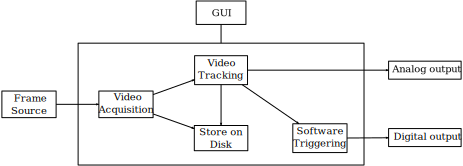
\includegraphics [width=\linewidth]{gfx/SpotterDesign.pdf} % [width=\textwidth]
	\caption[Test]{Design outline for online video tracking with physical output.}
	\label{fig:design}
\end{figure}

The goal is to provide a system that can bridge the gap between video streams with high information density to defined physical outputs based on flexibly adjustable criteria.

To provide a hardware interface that can be interpreted by experimental setups the system should give out pseudo-continuous signals as analog voltage values. These can be used for analog thresholding and filtering or by more proficiently by systems with analog-digital converters (ADCs). Secondly, digital outputs should provide signals for fast triggering based on selectable conditions minimizing computational load downstream. This reduces complex states down to binary signals. These signals, analog and digital, should be externalized in a way suitable for simultaneous monitoring on common electrophysiology data acquisition systems.

	To prevent data loss in case of improper set up and for offline analysis in general, the video data, detections and trigger events as well as the parameter states should be recorded suitable for archiving and fault tracing \ref{fig:design}.

Most commercially available consumer hardware provides video signals at 30 frames per second. This is sufficient for a large range of tasks. The delay between image acquisition and signal emission should be low enough to provide feedback within a theta cycle, as demanded by the experiment originally starting development.

Software and hardware should be easy to obtain, inspect, set up and modify  without advanced knowledge.

\newpage
%##############################################################################
\section{Implementation Considerations}
\label{sec:implementation}
%##############################################################################
	\subsection{Software}
	Many researchers are familiar with the MATLAB numerical computing environment (The MathWorks). MATLAB has support for image processing and can interface cameras through the Image Acquisition Toolbox. However, MATLAB and its toolboxes are expensive, building graphical user interfaces can be a jarring experience and is a rather bulky application.
	
	The most widely used library for computer vision is OpenCV. The open source framework is available for all major operating systems (Windows, Linux, OSX and iOS). While originally a C/C++ library, bindings for other languages are available (e.g. Python, Java). The library provides basic handling of input and output of image data (image and video files, many camera devices, streams) via the FFMPEG or GStreamer libraries at high de- and encoding speeds. OpenCV also exposes basic graphical user interface (GUI) methods for prototyping and a large number of numerical methods for most routine computer vision and machine learning tasks.
	
To make the resulting code of this project accessible for modification and maintenance, I decided to use the Python language bindings over C/C++ or Java. Python is a popular \cite{Tiobe} open source general purpose programming language that is easy to learn, has a focus on readability, can be used to write self-documenting code and is highly extensible. The SciPy/NumPy libraries provide mature support of numerical computation, linear algebra and machine learning. More importantly, recent OpenCV Python bindings are based on the linear algebra methods provided by NumPy. Several Python distributions focused on scientific computing (e.g. Enthought, PythonXY, Anaconda) provide bundles of the core requirements with integrated development environments (IDEs). This provides familiarity to MATLAB users while offering the advantages of a general purpose language. However, Python is a dynamically typed interpreted language. It is often slower than compiled languages (e.g. C/C++), although a number of ways exist to alleviate this difference (see section \ref{sec:discussion}). Modern multi-core desktop computers should nevertheless have enough computational capacity to allow realtime processing of video at moderate frame rates ($\leq 60$ fps) and resolutions even in this non-optimal case.

	\begin{listing}[t]
	\inputminted[%mathescape,
							 bgcolor=LightGrey,
               linenos,
               numbersep=5pt,
               %gobble=2,
               frame=lines,
               framesep=2mm]{python}{example.py}
	\caption{A minimal example of using the OpenCV Python bindings to receive and display frames from a video source. The library is imported and a video capture object created. The while loop is querying the capture object for new frames every \SI{30}{\milli\second} until a key is pressed.}
	\label{lst:pymin}
	\end{listing}
	
In listing \ref{lst:pymin} a minimal example of Python code is provided. The script uses the OpenCV library to open a video stream, here from a device with $id = 0$ (for example a camera) and displayed at 30 fps until the user presses a key. This example uses the basic interface methods provided by OpenCV to draw the frame. However, these methods are insufficient for building a more advanced graphical user interfaces. Instead, the Spotter user interface is built with the open source Qt library. It is available on most platforms, has a large range of language bindings including C/C++ and Python, carries no license fees for non-commercial applications and is used by a number of common neuroscience tools (e.g. NeuroScope, NDManager, KlustaViewa). 

Qt provides development tools to quickly build the layout (e.g. Qt Designer) and store these definitions in a language independent format separating structure and function. This way existing user interface designs can be ported quickly between different language implementations. This allows to transfer existing GUI designs from one language implementation to another. If the Python bindings of OpenCV turn out to not provide the required performance, this would greatly ease the transition to a C/C++ implementation.

	\subsection{Hardware}
	Three hardware building blocks are to be considered. Firstly, the video source device. While the system should be able to process video files for offline analysis, for realtime applications a low latency video stream of the subject to track is required. OpenCV provides a versatile \texttt{VideoCapture} (as well as \texttt{VideoWriter}) method that uses the FFMPEG multimedia library to decode video device streams from IP-cameras and USB-cameras compatible with the UVC (USB video device class) standard. Consumer-grade USB 2.0 camera devices are typically limited in resolution, frame rate and image quality, especially under poor lighting conditions. For many experiments a temporal resolution of less than \SI{30}{\milli\second} is sufficient, and tracking can be simplified by if animals carry easy to track hardware (like LEDs). Professional computer vision cameras (e.g. PointGrey Gigabit Ethernet/USB3 devices) can go beyond these basic parameters, but may not be supported by the OpenCV frame aquisition methods as they often require the use of vendor specific SDKs. Python is able to interface with external modules written in C, allowing the integration of these devices with moderate effort if needed.
	
This software was developed using USB2.0 attached LifeCam Studio 1080p HD Webcam (Microsoft) cameras. They have good resolution and reasonable image quality at a moderate price (\$75 at the time of writing). However, USB2.0 is fairly bandwidth limited (480 Mbps in theory) for high definition video. When purchasing a new camera, more recent standards (USB3.0, Thunderbolt) should be preferred, and are increasingly common.
	
Secondly, A desktop computer or laptop is used as the main processing device. While being the central device in the framework, its requirements are rather loose. A fairly modern computer ($<5$ years old) has sufficient processing power and connectivity (USB). All libraries used are available on the major operating systems (Microsoft Windows 7, Linux 2.7+, Apple MacOSX) and the software has successfully been tested on all of them (however, the installation process is easiest on up-to-date distributions, and most involved on Apple machines),
%, but Apple devices have had a much more involved installation process and were tested least.

A microcontroller is used to produce the physical output signals. While most PCs possess some ability to generate digital and analog signals (parallel ports, sound devices) they are limited in the number of channels, increasingly rare and burdened by other limitations (high-pass filters, difficult to control reliably). Microcontrollers are devices independent from the main processing machine (the PC) which are controlled via serial interfaces. A large variety of microcontroller ecosystems exist, but most have complicated toolchains, require familiarity with the underlying architecture and an intimate relationship with their datasheets or the assembly of the required peripherals. One of the most popular beginner-friendly ecosystems is the Arduino platform, providing open source hardware and software together. Its central element is a standardized range of microcontroller boards, typically based on 8 bit microcontrollers (AVR ATmega328; Atmel). These are available from a large number of distributors word-wide (\$20-50). The standard board implementation has USB connectivity and is pre-programmed with a bootloader which handles USB communication and acts as the self-programming in-circuit serial programmer (ICSP). The second component of the Arduino platform are an IDE that acts as a multi-platform toolchain to compile programs for the microcontroller, and a universal device driver. Typically microcontrollers are programmed using very low level languages, C or assembly, and require the user to reach an advanced understanding of the hardware. Arduino uses an abstraction and superset of C, providing higher-level access to the most common functions and applications. Additionally a large number of libraries for common devices and applications exist, in addition to beginner friendly learning resources. In summary, the Arduino microcontroller platform allows to easily read and write programs to be run on standardized hardware, optionally interfaced through a via USB connection from a host computer.

\newpage
%##############################################################################
\section{Implementation}
%##############################################################################
\begin{figure}%[] %hb
	\centering
		\includegraphics [width=\linewidth]{gfx/SpotterImplement_noInput.pdf} % [width=\textwidth]
	\caption[Test]{\texttt{spotterQt} is the graphical user interface based on the Qt framework. It wraps around the core \texttt{spotter} module to provide interactive control and visual feedback. The core module consists of four sub-modules, separated by task. The frame \texttt{Grabber} handles the capture object and returns a new frame when called. The \texttt{Tracker} uses defined feature sets to track the position of objects in the frames. For example bright spots from the position LEDs on the implant of a laboratory rodent. The position data is processed and defined results sent through the \texttt{Chatter} module over a serial connection to an Arduino microcontroller, which provides digital or analog output of the data. Frame and position data are stored on disk by a \texttt{Writer} module as compressed video and text log files. The writer is running in a separate process (dashed box) to provide data-handling without blocking the main thread.}
%Sensor data handling is incomplete at the time of writing (dashed arrows).

%The \texttt{Chatter} module can also receive sensor data from the microcontroller, like sensor crossings and other experimental variables.
	\label{fig:implement}
\end{figure}

\subsection{The \texttt{spotter.py} main loop}
The main loop of the script, referred to as the \texttt{spotter} module, can be run independently from the graphical user interface. This provides command line functionality to run headless on a server or be controlled from a remote machine. Additionally, this allows offline batch processing of recorded video data. Each loop iteration processes one frame from the video source, except when processing is paused. Within the \texttt{spotter} module, the core functionality is handled by four sub-modules, instances of the aptly named \texttt{Grabber}, \texttt{Tracker}, \texttt{Chatter} and \texttt{Writer} classes (Figure \ref{fig:implement}).


\subsubsection{Grabber}
\label{sec:Grabber}
The \texttt{Grabber} initiates, handles and holds the frame source (either a camera device or a video file) capture object reference (\texttt{vc} in Listing \ref{lst:pymin}). Many cameras compress frames and encode them in color spaces other than RGB to overcome bandwidth limitations. Grabber reads and decodes new frames. OpenCV returns a boolean return value if a frame was read successfully, and a 3-dimensional NumPy array. The array contains a 2D array slice with $width~x~height$ pixel elements for each of the RGB (red, green, blue) color channels. The elements of the array are stored as unsigned 8-bit integers (uint8), ranging from 0 to 255. Together, each pixel is can be represented by 24 bit RGB value, which OpenCV handles in B-G-R order. For futher processing, these arrays can be accessed and handled like typical objects in numerical computation software.

\begin{figure}%[ht] %hb
	\centering
		\includegraphics [width=\linewidth]{gfx/HSV-RGB-comparison_formula.pdf} % [width=\textwidth]
	\caption[Test]{RGB to HSV color space conversion. \emph{Left:} Ranging of HSV values wraps around the origin if stepping over red (hue 0). \emph{Right:} Formula for the conversion of RGB values to the cylindrical HSV color space.}
	\label{fig:HSV}
\end{figure}

Follow frame acquisition several pre-processing steps might be necessary. To reduce computational load images can be scaled, as the number of pixels decreases with the square of the scaling factor. Cheap consumer-grade cameras are noisy, especially under low light conditions. Low-pass filtering and and morphological operations are common pre-processing steps that can emphasize features of interest. They require careful use, however, as they tend to be computationally expensive and can reduce the signal fidelity. Example steps include smoothing (removes high frequency noise), dilation (exaggerates foreground features) and erosion (decreases features from their boundaries). Depending on the tracking algorithm employed, the frame may have to be converted to a suitable color space.%to HSV (Hue, Saturation, Value).

The features typically tracked in the intended application consists of brightly colored spots of the LEDs attached to the headstage of implants on laboratory rodents. Using RGB values however, these properties are not immediately accessible. Separation by the independent color channel values alone is often impractical. A bright red pixel (e.g. R=255, G=110, B=110) has a higher blue component than a dark blue pixel (e.g. R=0, G=0, B=100). More generally, the brightness, saturation and color are setting the off from the background (Figure \ref{fig:frames}). To easily access these features, the frames are transformed from the RGB to the HSV color space (Figure \ref{fig:HSV}). HSV is a cylindrical three channel color space. Hue (color tone) is encoded in a circular mapping, and value (brightness) and saturation (color intensity) are encoded linearly. Commonly the hue range is defined between $0-360^{\circ}$. However, the image data is stored as 8 bit values per channel. To fit the hue value into this range, OpenCV represents the hue space as half values ranging from 0 to 179. Distinctly colored pixels with defined saturation and brightness can now be separated by simple thresholding operations on the corresponding channels.

\begin{figure}[ht] %hb
	\centering
		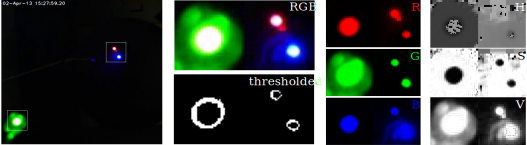
\includegraphics [width=\linewidth]{gfx/HSV_conversion.pdf} % [width=\textwidth]
	\caption[Test]{Example image of colored LED spots. \emph{Left:} Example frame with a green LED for synchronization, and two LEDs (red and blue) carried by the animal. \emph{Center top:} Magnified RGB image of the three spots. \emph{Right:} The separate R, G and B channels before, and separate H, S and V channels after the color space conversion. \emph{Center bottom:} Binary masks after each spot had thresholds applied to saturation and value. As center pixels are overexposed, they have no meaningful hue value and have to be excluded.}
	\label{fig:frames}
\end{figure}


\subsubsection{Tracker}
\label{sec:Tracker}

Three helper classes (features, regions of interest, objects of interest, defined as \texttt{Trackables}) are used as representations for different objectives.

\paragraph{Features}
\label{sec:Features}
Features are the elementary unit for tracking and represent descriptive sets of parameters. These are used by the appropriate tracking algorithm to find the feature in frames. For LEDs, the typical use case in this project, these sets are hue, saturation and value ranges, as well as maximum and minimum area constraints. Additionally, features can be flagged as static or moving (for example a synchronization LED appears at a fixed location) by the user. %, and search can be restricted to a region of interest (ROI) to reduce the computational load.

\paragraph{Region of Interest}
\label{sec:RegionOfInterest}
Regions of interest (ROIs) are parts of the image that can interact with Objects for conditional signaling. ROIs consist of one or more geometric shape descriptors. Shapes (rectangles, circles, lines, polygons) consist of at least two points. The shape type defines how the points are interpreted. ROIs can be linked with Objects, and each Object/ROI connection tied to a physical output pin on the microcontroller. Collision or traversal of the Object through a linked ROI triggers a state change on the associated digital channel.
%(Figure \ref{fig:ROIs})


\paragraph{Objects of Interest}
\label{sec:ObjectsOfInterest}
% Normal vector with three features???? Maybe have an arbitrary axis and have all features relative to that axis. As long as two features exist, direction can be calculated.
Objects of interest (OOIs, the name is chosen to separate the naming from programmatic objects) are representations of real-world objects to be tracked. Objects consist of a set of one or more features. For example the subject in figure \ref{fig:frames} is represented by two features, one for a red, and one for a blue LED. A second object, the synchronization LED, is represented by a single static green LED feature. After all active features have been tracked (returning either coordinates or \texttt{None}) the position of an OOI is calculated as the mean of all its linked features. If no feature of the Object was detected, the position of the Object for that frame becomes \texttt{None}. This allows distinction of a zero position from a tracking failure in the output signals. From the history of positions a range of parameters can be calculated. For single frames, Objects with multiple features can have a direction of an arbitrary axis, calculated as the normal vector of two of its features. For multiple frames, velocity and acceleration can be computed. These values, together with digital triggers based on the collision with specified ROIs, can be sent to the microcontroller to be represented as digital or analog electrical signals.


\begin{figure}%[] %hb
	\centering
		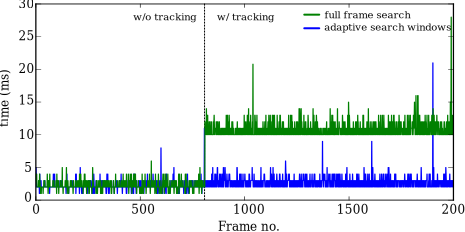
\includegraphics [width=\linewidth]{gfx/tracking.pdf} % [width=\textwidth]
	\caption[Test]{Tracker computation time for HSV thresholding operation is greatly reduced for adaptive region of interest constrained search. Tracking was started at dashed line. With adaptive search windows (blue) tracking time only slightly increases over pre-processing time. Without search constraints total tracking time is four times higher (green).}
	\label{fig:tracking}
\end{figure}

\paragraph{Tracking}
\label{sec:Tracking}
The \texttt{Tracker} iterates over a list of features. For the purpose of this report, I will limit the description to simple tracking by application of thresholds in the HSV space. 

To reduce the time spent on this step, a simple adaptive search window is applied by slicing the frame array during tracking. The window is calculated by stepping through the position history until a valid position is found. Centering on this position a rectangle is set up, increasing in size with the number of invalid positions preceding the valid one. This incrementally expands the window if a feature is lost. In the current state of development, not using information about directionality, velocity or acceleration or other prediction improvements to further reduce window sizes, this yields dramatically reduced search times for features with reliable detection. For example in figure \ref{fig:tracking} three LEDs are tracked with minimally $100\times100~px^2$ windows from $640\times360~px^2$ frames. The time per iteration is reduced from 11 ms to under 3 ms, including the unchanged pre-processing fixed time costs.

A binary mask array of pixels matching the feature description is created (Figure \ref{fig:frames}, bottom center). The element-wise application of range thresholds onto the three color channels of the converted frame array yields three binary arrays which are joined with the AND operator. To find contiguous pixel areas, a border following algorithm extracts contours \cite{Suzuki1985}. The first raw moments ($m_{ij}=\sum_{x,y}(frame[x, y] \cdot x^i \cdot y^j)$) are used to calculate the area ($m_{00}$) and the centroid for contours within the maximum and minimum area ($\bar{x} = \frac{m_{10}}{m_{00}} , \; \bar{y} = \frac{m_{01}}{m_{00}}$). The resulting coordinates of the contour with the largest area represent the geometric center of the detected pixel group for the feature.

A drawback of the naive thresholding method for detection colored pixel groups is the flooring effect of over-exposed values. The RGB to HSV conversion algorithm can not return meaningful values of the hue if all color components are equally present, and defaults to zero (red). This equates to the longitudinal axis of the color space cylinder (Figure \ref{fig:HSV}). For the most part these are rare cases and can be ignored. However, if the brightness of a light source saturates the image sensor, these pixels will be whitened, and fall back to Hue value of zero when converted to the HSV color space. To avoid this, the upper limit of the Value channel is set close to this maximum, and white pixels are ignored. This can lead to ring-shaped contours being found if performed aggressively (Figure \ref{fig:frames}, bottom center). For the calculation of the centroid this is of minor importance and will be accepted. It is preferable to have slightly reduced tracking precision over missing the spot altogether. A second drawback is the ranging over intervals crossing the origin (e.g. compare Range 1 and 2 in figure \ref{fig:HSV}, top) wraps around. This requires to either perform two operations of the two sub-intervals, or one operation of the inverted interval and the negation of the returned mask. Depending on the implementation of the ranging operation (separate or combined iteration over channels), either can be advantageous.

If no valid position for a feature is found at a time point, the Python NULL value \texttt{None} is returned instead, to distinguish numeric values from the fault case.

\subsubsection{Chatter}
\label{sec:Chatter}

The \texttt{Chatter} module handles all connectivity with the microcontroller. Most importantly it holds and wraps reference to the instance of an \texttt{arduino}-class that takes care of low-level communication and opening the serial port connection by bootstrapping the \texttt{pySerial} library. Establishing the connection requires finding the port the microcontroller is connected to, which varies greatly between operating systems. Excluding unlikely ports (e.g. Bluetooth serial devices) ports are scanned during automatic port selection by opening and polling all listed ports sequentially. If the right port is found, the microcontroller will respond with a fixed message. To further validate the connection, a handshake is performed. First, \texttt{Chatter} will send a string of data which will be mirrored back by the controller. If the send-and-receive test was successful, the microcontroller will report the device capabilities (number of DAC, digital output, digital input and PWM pins).

After each frame was processed and features/objects were tracked, selected signals (see the interface section (\ref{sec:GUI}) on linking detections with signal pins) are transmitted to the microcontroller using a simple instruction-data protocol. A four byte packet is sent for each signal per frame, consisting of one instruction byte and two data bytes, followed by a newline symbol (Figure \ref{fig:protocol}). The last byte marks the packet end, adding redundancy to allow recovery from packet alignment loss. The instruction byte contains 3 address bits and 3 type bits indicating the signal type (e.g. an analog signal on DAC channel 2, see figure \ref{fig:protocol}). Two padding bits are filling the instruction to a full byte, adding debugging information and shifting the instruction to values representing human readable symbols in the ASCII table (e.g 'I', 2\textsuperscript{nd} DAC channel).

 %(analog out, digital in/out, PWM)

\begin{figure}%[] %hb
	\centering
		
\includegraphics [width=\linewidth]{gfx/protocol.pdf} % [width=\textwidth]
	\caption[Test]{Structure of a four byte example packet employed in the Spotter-Arduino communication protocol. The example sets DAC 2 to 2.1 V (Figure \ref{fig:DAC}, right).}
	\label{fig:protocol}
\end{figure}

%This module is also responsible for receiving data. The microcontroller can function as a remote sensing unit. This way sensor data (e.g. data from position sensors, online spike sorting and other feedback modalities) can be integrated and displayed in context of the video frame. However, this functionality is unfinished.

%\subsection{Signal IO}
%\label{sec:IO}

\paragraph{Analog output}
\label{sec:AnalogOutput}

\begin{figure}%[] %hb
	\centering
		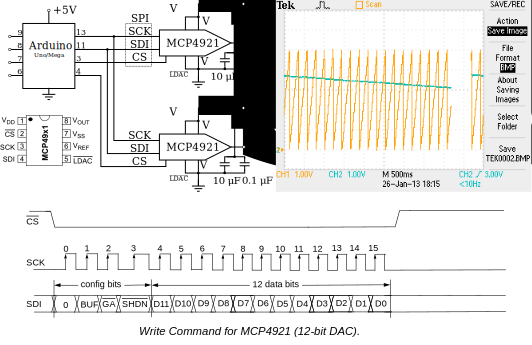
\includegraphics [width=\linewidth]{gfx/circuit.pdf} % [width=\textwidth]
	\caption[Test]{Arduino and DAC connections. \emph{Top left:} Two MCP4921 12 bit DACs are interfaced to the Arduino via SPI protocol, requiring two common lines for clock and data signals, and one line per device for destination selection. \emph{Top right:} Screenshot of a test pattern, quickly scanning the available range. Data is sent from a python program to the Arduino, which updates the DAC values accordingly. \emph{Bottom:} SPI protocol for the MCP4921 DAC. 2 bytes (12 data bits, 4 configuration bits) are sent aligned to the clock line, when the device selection line (CS) for the specific DAC is pulled low. Voltage values are updated immediately when a valid write command is received, as the LDAC buffer pin is permanently pulled low.}
	\label{fig:circuit}
\end{figure}

\begin{figure}%[] %hb
	\centering
		\includegraphics [width=\linewidth]{var/Spotter_bb.png} % [width=\textwidth]
	\caption[Test]{Schematic of the assembled hardware. \emph{Left:} Arduino Uno microcontroller board. The Arduino is connected to a PC via USB and provides regulated power, SPI data to the DACs (CS: blue/orange; SCK: yellow; SDI: green) and digital trigger outputs (gray). \emph{Right:} Breadboard with wire connections and bypass capacitors to the MCP4921 DAC ICs producing analog output signals (Vout X/Y: violet).}
%	Two optional bypass capacitors (\SI{0.1}{\micro\farad} ceramic and \SI{10}{\micro\farad} tantulum) may reduce high-frequency noise in the
%\SI{5}{\volt} power (\SI{5}{\volt}: red; GND: black)
	\label{fig:hardware}
\end{figure}

Digital to analog conversion (DAC) of pseudo-continuous values (i.e. position, speed, head direction, acceleration) is performed by 12 bit DAC ICs (MCP4921; Microchip), interfaced by the microcontroller via SPI (Serial Peripheral Interface, for protocol details please see datasheet; Figure \ref{fig:circuit}). SPI is a bidirectional serial bus protocol with master-slave architecture. It requires at least three lines (four for bidirectional communication, not required for the DACs) for a clock line (SCK), and a master-to-slave data line (SDI). Additionally, for each slave device a single device-select line is required to address a data stream to a specific device (CS). The MCP4921 uses an external voltage reference (V\textsubscript{ref}), which is tied to the supply voltage, providing near rail-to-rail range (\SI{40}{\milli\volt} offset at both ends, effective $V_{range}$ of \SIrange{0.04}{4.96}{\volt} for a perfect \SI{5}{\volt} supply). Two optional bypass capacitors (\SI{0.1}{\micro\farad} ceramic and \SI{10}{\micro\farad} tantalum) close to the voltage supply of the DACs may reduce high-frequency noise in the output signals.

To convert the position to an analog voltage value, three conversation constants are computed based on the DAC specifications and the frame size. To clearly separate invalid values (e.g. position tracking failed), the zero position is offset by 1/16th of the range. First, the DAC factor converts pixels units to arbitrary DAC units: $(\max_{DAC}-\frac{\max_{DAC}}{16})\times \frac{1}{framesize_{\max}}$, with $\max_{DAC}=4095$ for a 12 bit DAC. A frame size of $640\times360$ pixel has a DAC factor of 6 units per pixel. A DAC unit is converted to voltage values by the factor $\frac{V_{range}}{\max_{DAC}}$, which in the case of MCP4921 and a \SI{5}{\volt} supply and reference voltage corresponds to \SI{1.2}{\milli\volt} per unit. In total, pixel values have \SI{7.2}{\milli\volt} resolution. To represent images with non-unary aspect ratios, the minor axis is translated into the space of the major axis, maintaining an absolute pixel-to-voltage ratio (Figure \ref{fig:DAC}).

\begin{figure}%[] %hb
	\centering
		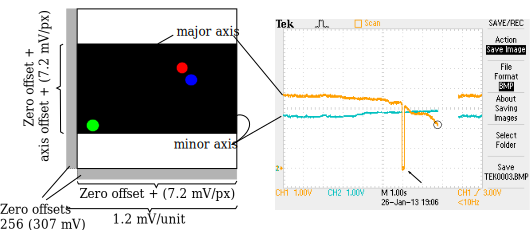
\includegraphics [width=\linewidth]{gfx/DAC_ranges.pdf} % [width=\textwidth]
	\caption[Test]{Conversion of image location to voltage values. \emph{Left:} Relation of frame to voltage values. \emph{Right:} Example screenshot of the analog position signal (x: orange, y: blue), as the animal is starting to traverse the arena after the half mark. Shortly after tracking is lost for a frame and the signal defaults to a fault value (arrow). The example value of previous figures is shown as the current state of the major axis signal (circle).}
	\label{fig:DAC}
\end{figure}

\paragraph{Digital output}
\label{sec:DigitalOutput}

Digital signals are updated in a straight-forward update loop. Each frame all digital pins are updated to either HIGH or LOW states. In the current version, a full packet is sent per digital pin. All non-zero data values are interpreted as HIGH, zero-data as LOW.

\subsubsection{Writer}
\label{sec:Writer}
To store experimental data for offline analysis, the video stream can be stored as a compressed video file (codec choice depends on the installed OpenCV backend), together with a log file of timestamped position and event data. Writing to hard drives can cause blocking long-latency operations, especially if other processes are accessing the hard drive with long seek times (e.g. the computer is performing electrophysiology data acquisition in parallel). To prevent the main process from waiting for video data to be written, \texttt{Writer} is running as a separate process. To maintain thread-safety, the inter-process communication is handled by two queues, allowing the exchange of control messages and data.

\subsection{User Interface}
\label{sec:GUI}

The user interface was designed with Qt Designer, which produces language independent definitions. These were translated into Python code. The resulting modules are the structural description of the interface components. These were linked with functional code, defining the behavior of the interface elements. In its current state, starting the program requires providing information via command line parameters, most importantly the frame source origin. As Spotter is intended to be operable purely as a command line tool, interface equivalents are added successively, but as a secondary priority.

The core element of the interface is an OpenGL context, displaying the video frames as they are grabbed from the frame source. As frames captured by OpenCV are NumPy arrays, frames had to be transformed to be accessible by OpenGL without major performance hits. This is achieved by casting the whole arrays into strings and using the OpenGL \texttt{DrawPixels} method to read these strings as byte strings. The OpenGL frame also handles user input (mouse and keyboard) to allow interactions with the video frame (e.g. drawing and moving ROIs, selecting areas to extract features from). Onto the OpenGL frame, frame-context interface elements are drawn (ROIs, tracking markers, debugging information) using OpenGL primitive methods. Currently, rendering and processing are performed sequentially.


\begin{figure}%[] %hb
	\centering
		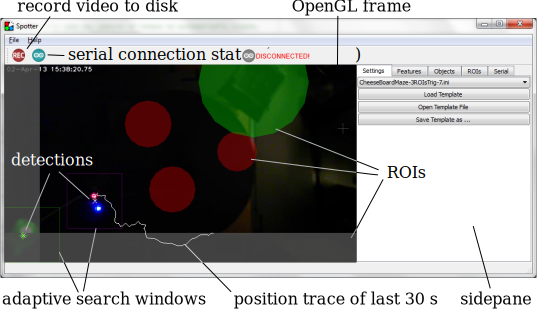
\includegraphics [width=\linewidth]{gfx/GUI_overview.pdf} % [width=\textwidth]
	\caption[Test]{Overview of the Spotter GUI elements.}
	\label{fig:GUI_overview}
\end{figure}

I will refrain from detailing the user interface, but give a short overview of its main use pattern. In brief, the typical workflow starts by establishing a connection of the program with the microcontroller, which can happen automatically, or require manual adjustment of the connection parameters (Figure \ref{fig:workflow}, A). To prevent data loss, a clearly visible indicator in the toolbar shows the current connection status (Figure \ref{fig:GUI_overview}, top). Next, features are added and adjusted to yield robust tracking performance (Figure \ref{fig:workflow}, B and C). Secondly, objects are added and linked with one or multiple features (Figure \ref{fig:workflow}, D and E). Object positions are calculated as the mean position of all its linked features. As long as free devices are available, object properties can be tied to analog output slots (Figure \ref{fig:workflow}, F). Next, regions-of-interest are added. Each ROI can consist of multiple geometric shapes (Figure \ref{fig:workflow}, G and H). To allow conditional triggering, objects and regions-of-interests can interact. ROIs can be linked with objects, and collision of ROI and object trigger digital output pin transitions (Figure \ref{fig:workflow}, I).

\begin{figure}%[] %hb
	\centering
		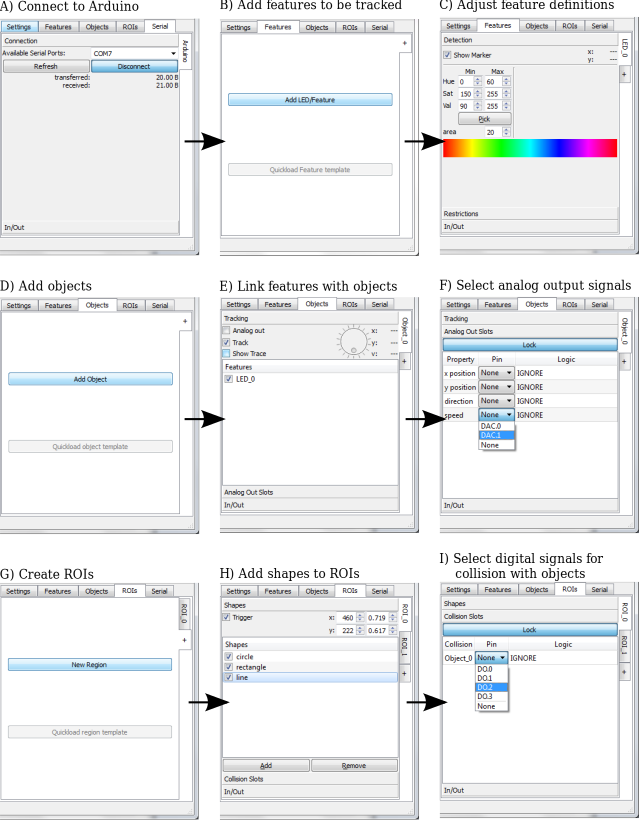
\includegraphics [width=\linewidth]{gfx/workflow.pdf} % [width=\textwidth]
	\caption[Test]{Simplified workflow to set up a new experiment.}
	\label{fig:workflow}
\end{figure}

Once the tracking and triggering is set up with, settings can be stored as template files for easy recovery and offline analysis (not shown). During the experimental run, video data, position and event logs can be written to the hard drive by toggling the record button (Figure \ref{fig:GUI_overview}). During writing, a timestamp is added to the video frame, additionally to the timestamps in the log files. 

\newpage

%##############################################################################
\section{Results}
\label{sec:results}
%##############################################################################

Online video tracking with Spotter is now actively and routinely used in Prof. Buzsaki's group to trigger optogenetic stimulation for closed-loop experiments (Figure \ref{fig:dmax}). As the application is under development, several bugs exist, and the hardware is not finalized. Initial analysis of the spatial and temporal characteristics shows good spatial, but limited temporal precision.% but which can be improved in several aspects.

\begin{figure}%[] %hb
	\centering
		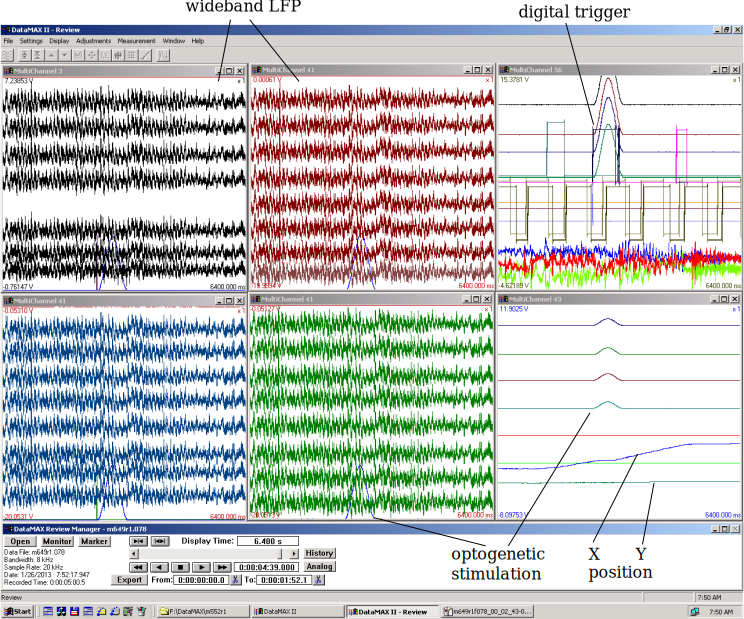
\includegraphics [width=\linewidth]{gfx/dmax_example.pdf} % [width=\textwidth]
	\caption[Test]{Example screenshot of position triggered optogenetic stimulation together with 32-channel wideband LFP signals. Position data is additionally to the digital triggered recorded as an analog voltage value (blue and green traces, lower right corner).}
	\label{fig:dmax}
\end{figure}


\begin{figure}[ht] %hb
	\centering
		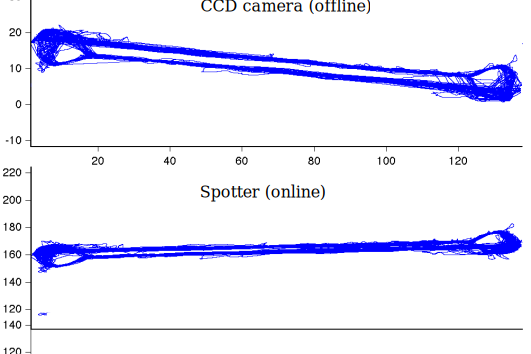
\includegraphics [width=\linewidth]{gfx/cameras.pdf} % [width=\textwidth]
	\caption[Test]{Comparison of offline computed position with Spotter position tracking as computed from the analog position signal recorded concurrently with the electrophysiology data acquisition system. (units are arbitrary (CCD camera) or pixel (Spotter))}
	\label{fig:cameras}
\end{figure}

\subsection{Spatial precision}
\label{sec:SpatialPrecision}

While the spatial resolution is on the order of the frame resolution if the image was not scaled for tracking, the effective precision greatly depends on the tracked feature and the feature definition. Partial detection, caused for example by overlap of the tether with an LED, complete coverage and failed detection, as well as partial rejection of the feature due to overexposure or improper parameter definitions can cause small changes in the computed position of objects. For objects with multiple features, failed detection shifts the mean position and can cause jitter in the signal. Compared to the offline analysis of the previously used camera, Spotter yields highly coherent data compared to the same experiment recorded with a CCD camera (Figure \ref{fig:cameras}). Both show near identical movement patterns, even though they have been recorded from slightly different angles.
%, showing that Spotter online detection is at least as good as offline detection used before


\subsection{Temporal precision}
\label{sec:TemporalPrecision}

The temporal properties of the online system have to be measured relative to a signal with high temporal precision. In figure \ref{fig:temporal} the signal of a green flashing synchronization LED is tracked by having an object, linked to a single feature, collide with a ROI. Upon collision detection, a digital pin of the Arduino is updated after transmission via serial port. This allows precise estimation of the detection and triggering delay. Measuring the peak cross-correlation shows about 109 ms in lag between the current applied to the LED and the digital signal being recorded.

\begin{figure}[H] %hb
	\centering
		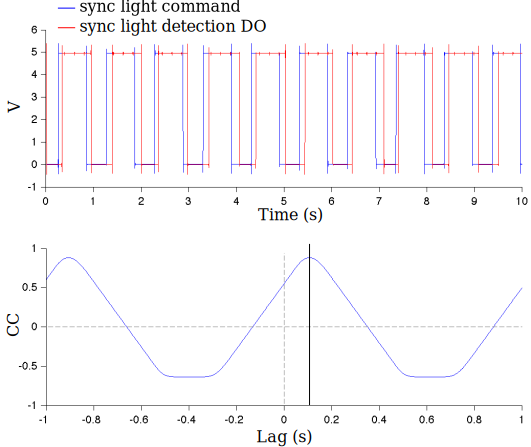
\includegraphics [width=\linewidth]{gfx/temporal.pdf} % [width=\textwidth]
	\caption[Test]{Temporal correlation between monitored current of a flashing synchronization LED and digital signals emitted by Spotter detecting the light. \emph{Top:} Time course of the signals. The digital signal of Spotter lags behind the actual current applied to the LED. \emph{Bottom:} Cross-correlation of the two signals. The Spotter signal lags by about 109 ms. [NOTE: These values are based on an older version with timing issues. Current HEAD measures loop lag of approximately 50 ms]}
	\label{fig:temporal}
\end{figure}

\newpage
%##############################################################################
\section{Discussion}
\label{sec:discussion}
%##############################################################################
In the current state of development Spotter allows robust video tracking of laboratory rodents. While designed for animals carrying hardware (i.e. head mounted LEDs), tracking is generalizable for any object which can be distinguished within the HSV color space. Furthermore, multiple objects can be tracked independently at the same time. By reducing the search window dynamically, additional features add little computation time and the tracking delay is dominated by fixed components of the analysis pipeline. In future iterations of the software, the option to integrate modules with new features and tracking algorithms could greatly extent versatility and tracking performance.

For any system with a low sampling rate, delays are unavoidable. This is most obvious for binary signals like flashing LEDs, where the timing of frame acquisition to signal onset is critical. In the worst case, the LED lights up during frame acquisition, leading to incomplete exposure and missing the light although already visible in the frame, adding another full frame length to the detection time (e.g. 33 ms at 30 fps). In the best case, the signal light is active just before frame acquisition. This jittering can only be improved by an increase in frame rate, or by triggering frame acquisition on external signals correlated with the feature of interest (e.g. current applied to the LED).

For continuous signals however, this limitation is of less importance. Here, the buffer and processing delay is critical. The reported lag times are for an older version of the program not using adaptive search windows. One can expect from the decrease in processing time by about 10 ms the cross-correlations to improve accordingly. However, this still leaves about 100 ms of delay. While experiments to pinpoint the origin of the delay are underway, I can speculate on the probable causes.

Using inexpensive video acquisition hardware like an off-the-shelf webcam is cheap, but comes with engineering trade-offs. To allow transmission of high-resolution video over a bandwidth limited port like USB 2.0, the video stream has to be encoded on the remote device. For this purpose, a framebuffer on the camera is likely holding at least one frame for subsequent encoding. At least one more framebuffer is employed by the video acquisition library, followed by a decoding buffer. Each of the buffers can increase the time between acquisition on the camera sensor to processing availability by a full frame length, e.g. 33 ms. Thus the buffering of three frames along the acquisition pipeline would fully explain the delay. Finding the location of the buffers could provide means to mitigate the lag. It is open whether the use of Python bindings versus the C/C++ interface introduces additional buffering delays, or whether buffering is dependent on the video acquisition backend used by OpenCV.  

While minor compared to the lag introduced by processing and data acquisition, the serial connection to the microcontroller can be improved. Several Arduino-compatible microcontrollers exist that use a 32 bit ARM based chip, instead of the 8 bit Atmel. These typically have much faster data transmission with lower latencies. Additionally, they are available with built-in DACs (e.g. Arduino Due), reducing the complexity of the hardware. The controller choice aside, the current protocol transmits a lot of overhead per packet. Two DAC channels can be served by a single packet and updating up to 8 digital pins requires a single byte of data. Using the padding bits and reducing the address/device type space to 2 bits each can free enough bits to allow packet length encoding, reducing the overall message length to 3 or 4 bytes. Combining digital and analog updates can result in a total message length of 5 bytes, at the cost of protocol flexibility.

The number of analog and digital channels used can easily be extended. Both the serial and SPI connection have sufficient bandwidth for dozens of devices and the communication protocols are designed with wide address spaces. Furthermore, the Arduino reports its hardware capabilities to the Spotter software. Adding new channels only requires adding the controlling pin to an array in the Arduino code and may be of use when tracking multiple objects.

The widespread introduction of multiplexed high-channel electrophysiology systems based on Intan hardware introduces new challenges for concurrent recording of electrophysiology and external signals, as these systems employ high pass filters (typically 0.1 Hz), rendering DC signals like the slowly changing analog output and rarely changing digital signals useless. To overcome the high-pass filter, multiple future options are under investigation. Primarily, signals can be alternated quickly using bipolar DACs. However, this would increase the difficulty of using these signals externally. Alternatively, encoding analog signals with digital patterns could sidestep high pass filtering using pulse modulation techniques (e.g. PWM, PCM, PDM). But all similarly increase the difficulty of using signals by components other than for mirroring. Likely, adding additional DAC channels to allow both, pure DC signals and coded signals to be emitted concurrently will be required. Additionally to the existing output states and devices, a useful addition would be the ability to encode arbitrary numerical variables as digital, and to a lesser extent analog, signals. As an example, encoding frame IDs as digital PCM or PWM patterns would allow precise alignment of video to electrophysiology recordings during offline analysis.

While the interface in general will require a lot of continued effort, a main step towards increased performance is to separate rendering and processing. Currently, these two are performed sequentially. Any delay in rendering can delay the processing of frames, including frame skips, reducing the temporal resolution and precision. As with the \texttt{Writer} module the \texttt{Grabber} could be placed into a separate process, or at least a separate thread. This can be generalized to a producer-multiple consumer architecture. Having a separate thread/process for these modules would allow to move between Python and C modules, the latter could provide a great boost to performance while keeping the ease-of-use of Python for the remainder of the code. Using C modules would also allow to integrate libraries to interface non-standard cameras that require vendor specific software development kits, like most cameras better suited for realtime computer vision than webcams. These can achieve higher frame rates (100 Hz and higher) at low latencies and well defined frame acquisition timings. Together with hardware triggering of shutter and sensor signal conversion, this could allow extremely low latency, high speed position tracking with the existing program.

\section*{Acknowledgements}
\label{sec:acknowledgements}
I greatly appreciate all the help I received in Prof. Buzs\`aki's group working on this project. Especially, I want to thank Eran Stark for technical advice. He created the figures for spatial and temporal correlation. And I want to thank Lisa Roux for suggestions and her thorough continuous beta (or rather alpha) testing. The example screenshot in figure \ref{fig:GUI_overview} is made with one of her recordings. Sven Ehrlich provided a long-term rental of his Arduino when mine was left behind in New York...
%
%A change in architecture aside, implementation of smarter tracking algorithms and additional feature types would expand the capabilities of the system. The current tracking algorithm is very simple and can easily be confused (being more detection than tracking).



%
%
%\section*{Section 1}
%
%\lipsum[1-3] % Dummy text
%
%\begin{align}
%A = 
%\begin{bmatrix}
%A_{11} & A_{21} \\
%A_{21} & A_{22}
%\end{bmatrix}
%\end{align}
%
%\lipsum[4] % Dummy text
%
%%------------------------------------------------
%
%\subsection*{Subsection 1}
%
%\lipsum[5] % Dummy text
%
%\begin{itemize}
%\item First item in a list 
%\item Second item in a list 
%\item Third item in a list
%\end{itemize}
%
%\lipsum[6] % Dummy text
%
%%------------------------------------------------
%
\clearpage
\section*{Appendix}
\label{sec:Appendix}


%\subsection{Bill of materials}
%\label{sec:BillOfMaterials}

\begin{table}[h]
\centering
	\begin{tabular}{rllr}
	\toprule
	%\multicolumn{2}{c}{Name} \\
	%\cmidrule(r){1-2}
	\# & Part name & Part \# & Price [\$]\\
	\midrule
	1 & Arduino Uno R3 & 78T1601  & $25.00$ \\
	1 & USB A to B cable & PSG90003  & $2.00$ \\
	2 & MCP4921 12 bit DAC & 08J8743  & 4.00 \\
	2 & \SI{0.1}{\micro\farad} ceramic capacitor & 97M4140 & 0.20 \\
	2 & \SI{10}{\micro\farad} tantalum capacitor & 25M8461  & 1.00 \\
	%var & wires & --  & -- \\
	%1 & breadboard & --  & -- \\
	%var & connectors (BNC) & --  & -- \\
	1 & Microsoft LifeCam Studio 1080p HD Webcam & --  & $50.00$ \\
	\bottomrule
	\textbf{Total} & & & \textbf{82.20}\\
	\end{tabular}
\caption{Bill of materials for a basic 2-channel implementation of the Spotter hardware. Part numbers are examples, retrieved July 2013 from newark.com. Does not include the PC required.}
\end{table}
%
%%------------------------------------------------
%
%\section*{Section 2}
%
%\lipsum[8] % Dummy text
%
%\begin{description}
%\item[First] This is the first item
%\item[Last] This is the last item
%\end{description}
%
%\lipsum[9] % Dummy text

%------------------------------------------------------------------------------
%	REFERENCE LIST
%------------------------------------------------------------------------------

\clearpage
\bibliographystyle{plain}
\bibliography{Spotter}
%------------------------------------------------------------------------------

\end{document}